\chapter{Bounding the synchronous flooding time}
\label{chapter:SyncFlooding}

In this chapter we consider a new algorithm for rumour spreading on dynamic network known as flooding, which takes place in discrete rounds instead of continuous time. First we introduce algorithm and prove an upper bound for the spreading time on a dynamic network from \cite{syncPaper}. Then we introduce a new type of dynamic network, where the sequence of topologies is not deterministic, but instead follows a distribution. We generalise our flooding bound to this probabilistic class of dynamic networks, and see an extended example of applying the bound.

\section{Model}

First we introduce a new algorithm for rumour spreading in discrete rounds (referred to in \cite{asyncPaper} as synchronous spread).

\begin{definition} \label{SyncFloodingAlgorithm}
	Synchronous Flooding Algorithm

	\noindent
	The synchronous flooding algorithm proceeds in rounds on a dynamic network $\mathcal{G} = (G_t)_{t \in \mathbb{N}}$. Initially a single node is aware of the rumour. In round $i$, every node that is aware of the rumour informs all of its neighbours in $G_i$, regardless of whether they already knew the rumour or not.
\end{definition}

We note that the asynchronous rumour spreading algorithm (Algorithm \ref{NodeCentricAsyncAlgorithm}) was probabilistic since the algorithm depended on sources of randomness such as exponential clocks. In contrast, once the dynamic network and initial node from which the rumour spreads are chosen, Algorithm \ref{SyncFloodingAlgorithm} is entirely deterministic. Since the trajectory of the rumour spread is completely determined by the initial conditions, it is reasonable to ask why we would want bounds on the spreading time if we can simply simulate the rumour, and record how long it takes to inform all the nodes. In some cases however, the graph may be so large that simulation is computationally infeasible. 
In such cases, we may be able to take advantage of bounds in terms of the structural properties of graphs instead. % TODO: Said "cases" at beginning of both sentances
Additionally, in Section \ref{section:MEDNBound}
we analyse rumour spreading on a non-deterministic dynamic network, where the sequence of graphs is not fixed but instead follows some distribution. 
In this case, deterministic bounds will allow us to bound spreading time over the distribution of graph sequences. %TODO: Said "case" again - change

% TODO: Why study flooding time?
% TODO: mention that Flooding only works for synchronus


\section{Bound on spreading time for the Flooding Algorithm}

In this section we prove a bound on the spreading time of the flooding algorithm from \cite{syncPaper}, adding details and expanding steps throughout.

First we introduce the notion of an expander graph, which we need to express the bound.

\begin{definition}
	Boundary set $B(S)$

	\noindent 
	Given a graph $G=(V,E)$, the boundary set $B(S)$ of a vertex subset $S \subseteq V$ is defined as the set of vertices outside $S$ connected to a node of $S$ by an edge, i.e
	$$
		B(S) = \left\{u \in V \setminus S : \{u, v\} \in E \text{ for some } v \in S \right\}
	$$
\end{definition}

% TODO: Figure of boundary sets

\begin{definition}
	$(h, k)$-Expander

	\noindent
	A graph $G$ on a vertex set $V$ is a $(h, k)$-expander if all subsets of the nodes $S \subseteq V$ such that $|S| \leq h$ satisfy $|B(S)| \geq k|S|$.
\end{definition}

Intuitively, an $(h, k)$-Expander should be well-connected since each "small" subset of nodes (i.e. less than $k$ nodes) is connected to at least $k$ other nodes outside the set.  

We are now ready give a bound on the rumour spreading time for the flooding algorithm.

\begin{theorem}\label{theorem:DeterministicFloodingBound}
	\ModelIntro Suppose also that there exists an increasing sequence $1 = h_0 \leq h_1 < \dots < h_s = \frac{n}{2}$ and decreasing sequence $k_1 \geq k_2 \geq \dots \geq k_s$ of positive real numbers, such that for all $t \in \mathbb{N}$, $G_t$ is a $(h_i, k_i)$-expander for every $i \in \{1, \dots , s\}$. Then the spreading time of $\mathcal{G}$ under algorithm \ref{SyncFloodingAlgorithm} is
	$$
		\mathcal{O}\left(\sum_{i=1}^s \frac{\log \frac{h_i}{h_{i-1}}}{\log(1+k_i)}\right)
	$$
\end{theorem}

% TODO: Interpretation of how the bound varies for different (h_i, k_i) sequences, how do these emerge?

We notice that there are strong conditions on the connectivity of the dynamic network that must be met for this bound to hold, namely that every topology is an $(h,k)$-expander for multiple $(h, k)$ pairs. Initially these conditions may seem unreasonably strong, however in Section \ref{section:floodingBoundEdgeMarkovian} we will see an interesting example where these properties emerge w.h.p in a random graph.

\begin{proof}
	For $i = 1,\dots, s$, let $T_i$ be the earliest time step such that the number of informed nodes is larger than $h_i$, i.e

	$$
		T_i = \min \{ t \in \mathbb{N} : |I_t| > h_i \}
	$$

	First we upper-bound the number of steps in the interval $[T_i, T_j]$, % TODO: Generalise to [T_i, T_j], should all hold as expected
	by bounding the number of informed nodes $t$ time-steps after $T_i$ from below.

	By induction, we show that if $T_i + t < T_j$, then the number of informed nodes at time $T_i + t$ is greater than $(1+k_j)^t h_i$.
	
	\underline{Base Case.} Suppose that $t=0$. 
	
	Then by the definition of $T_i$, the number of informed nodes at time $T_i$ is strictly greater than $h_i$

	\underline{Inductive Case.} For brevity, let $s = T_i + t$. Suppose that $|I_s| > (1+k_j)^t h_i$.

	We notice that 
	\begin{align*}
		|I_{s+1}| &= |I_s| + |B(I_s)| \\
		\intertext{by the operation of Algorithm \ref{SyncFloodingAlgorithm}}
		& \geq |I_s| + k_j |I_s| \\ % since we assume s < T_j => |I_s| \leq h_j + (h_j, k_j)-expander
		\intertext{as $G_t$ is a $(h_j, k_j)$-expander, so we observe that $|B(I_s)| \leq h_j$ since $s < T_j$}
		& = (1 + k_j)|I_s| \\
		& > (1 + k_j)(1+k_j)^t h_i \\
		\intertext{by the induction hypothesis}
		& = (1+k_j)^{t+1} h_i
	\end{align*}
	% TODO: boundary set picture here	
	Let $\tau = T_i + \ceil{ \frac{\log (h_j/h_i)}{\log(1+k_j)}}$. 
	Suppose for contradiction that $\tau < T_j$. %TODO: Is contradicition overkill here?
	Since we assumed $\tau < T_j$ we can apply the above inequality %TODO: label
	to get the following lower bound on the number of informed nodes at time $\tau$.
	$$
		|I_\tau| > 
		(1+k_j)^{\ceil{ \frac{\log (h_j/h_i)}{\log(1+k_j)}}} h_i
		\geq e^{\log (h_j/h_i)} h_i
		= h_j
	$$
	Thus we have a contradiction, since under the assumption that $\tau < T_j$, we get that the number of informed nodes at time $\tau$ is greater than $h_j$, i.e. by the definition of $T_j$, $\tau \geq T_j$. Hence, we have that $\tau \geq T_j$ i.e. $\ceil{ \frac{\log (h_j/h_i)}{\log(1+k_j)}}$ time-steps after $T_i$, the number of informed nodes is greater than $h_j$. Rearranging this inequality gives us the following bound on the length of the interval $[T_i, T_j]$:
	\begin{equation} \label{eq:FloodingIntervalBound}
		T_j - T_i \leq \ceil{ \frac{\log (h_j/h_i)}{\log(1+k_j)}} \leq \frac{\log (h_j/h_i)}{\log(1+k_j)} + 1
	\end{equation}
	% TODO: Make ceiling brackets fit
	% TODO: Exposition about next steps + direction here

	% TODO: What about time until first spread - must happen at timestep 2 since (h,k) expander so no isolated nodes.
	Note that since $h_s = \frac{n}{2}$, at time $T_s$ at least half of the nodes will be aware of the rumour. Hence, if we can bound $[T_0, T_s]$, we will have bounded the time it takes for half of the nodes to be informed. 

	To bound $[T_0, T_s]$, we bound each subinterval $[T_{i-1}, T_i]$. Naively applying the bound to each subinterval directly and taking the sum yields the overall bound 
	$$
		\mathcal{O}\left(\sum_{i=1}^s \frac{\log \frac{h_i}{h_{i-1}}}{\log(1+k_i)} + s\right)
	$$ 
	for the interval $[T_0,T_s]$. However, we can tighten the bound by removing the additive $s$ term through case analysis on the subinterval $[T_{i-1}, T_i]$, as follows.

	% TODO: Link back to theorem, after since n/2 = h_s, after T_s at least n/2 nodes are informed


	% TODO: Note that the source of the problems is the cieling function - aim to get into form like in thm statement, but can't naively add all togethe oterwise + O(S) error, requires deeper analysis

	\textbf{Case 1.} Suppose $\frac{\log (h_i/h_{i-1})}{\log(1+k_i)} \geq 1$.

	In this case $\frac{\log (h_i/h_{i-1})}{\log(1+k_i)}$ term is the dominant term in inequality (\ref{eq:FloodingIntervalBound}), thus
	$$
		T_i - T_{i-1} = \mathcal{O}\left( \frac{\log (h_i/h_{i-1})}{\log(1+k_i) }\right) + \mathcal{O}(1) = \mathcal{O}\left( \frac{\log (h_i/h_{i-1})}{\log(1+k_i) }\right)
	$$

	\textbf{Case 2.} Suppose $\frac{\log (h_i/h_{i-1})}{\log(1+k_i)} < 1$.

	In this case we cannot achieve the same bound on $T_i - T_{i-1}$, since the additive 1 is the dominant term. By following the same reasoning as in Case 1, instead we can only obtain that
	\begin{equation}\label{eq:Weak1StepBound}
		T_i - T_{i-1} = \mathcal{O}\left( \frac{\log (h_i/h_{i-1})}{\log(1+k_i) }\right) + \mathcal{O}(1) = \mathcal{O}(1)
	\end{equation}
	To understand the situation that this case represents, we inspect the inequality we assumed.
	By rearranging we find that $(1+k_i)h_{i-1} > h_i$. Since we have assumed that $T_{i-1} < T_i$, % TODO: Assume this earlier
	the number of informed nodes at the start of round $T_{i-1}$ satisfies
	$$
		|I_{T_{i-1}}| \leq h_i
	$$
	Hence, as the topology is an in $(h_i, k_i)$-expander, in round $T_{i-1}$ at least $|I_{T_{i-1}}|k_i$ new uninformed nodes on the boundary of the informed node set are informed. Thus, at the start of the next round, there are at least $(1+k_i)h_{i-1}$ informed nodes, since $|I_{T_{i-1}}| > h_{i-1}$ by the definition of $T_{i-1}$. Combining this with the rearranged form of the assumed inequality, we see that the number of informed nodes "jumps" to more than $h_i$ nodes in a single time step.

	It may be that after this jump there are also more than $h_j$ nodes for some $j \geq i$, %TODO: insert figure here of t vs |I_t|, for t = T_{i-1}, T_i, T_{i+1}, etc, maybe similar figure for steps in case 1.
	from which we obtain $T_{i-1} + 1 = T_i = T_{i+1} = \dots = T_j$. See Figure \ref{fig:floodingJump} for an illustration of this "jump" behaviour. 
	\begin{figure}[h]
		\centering
		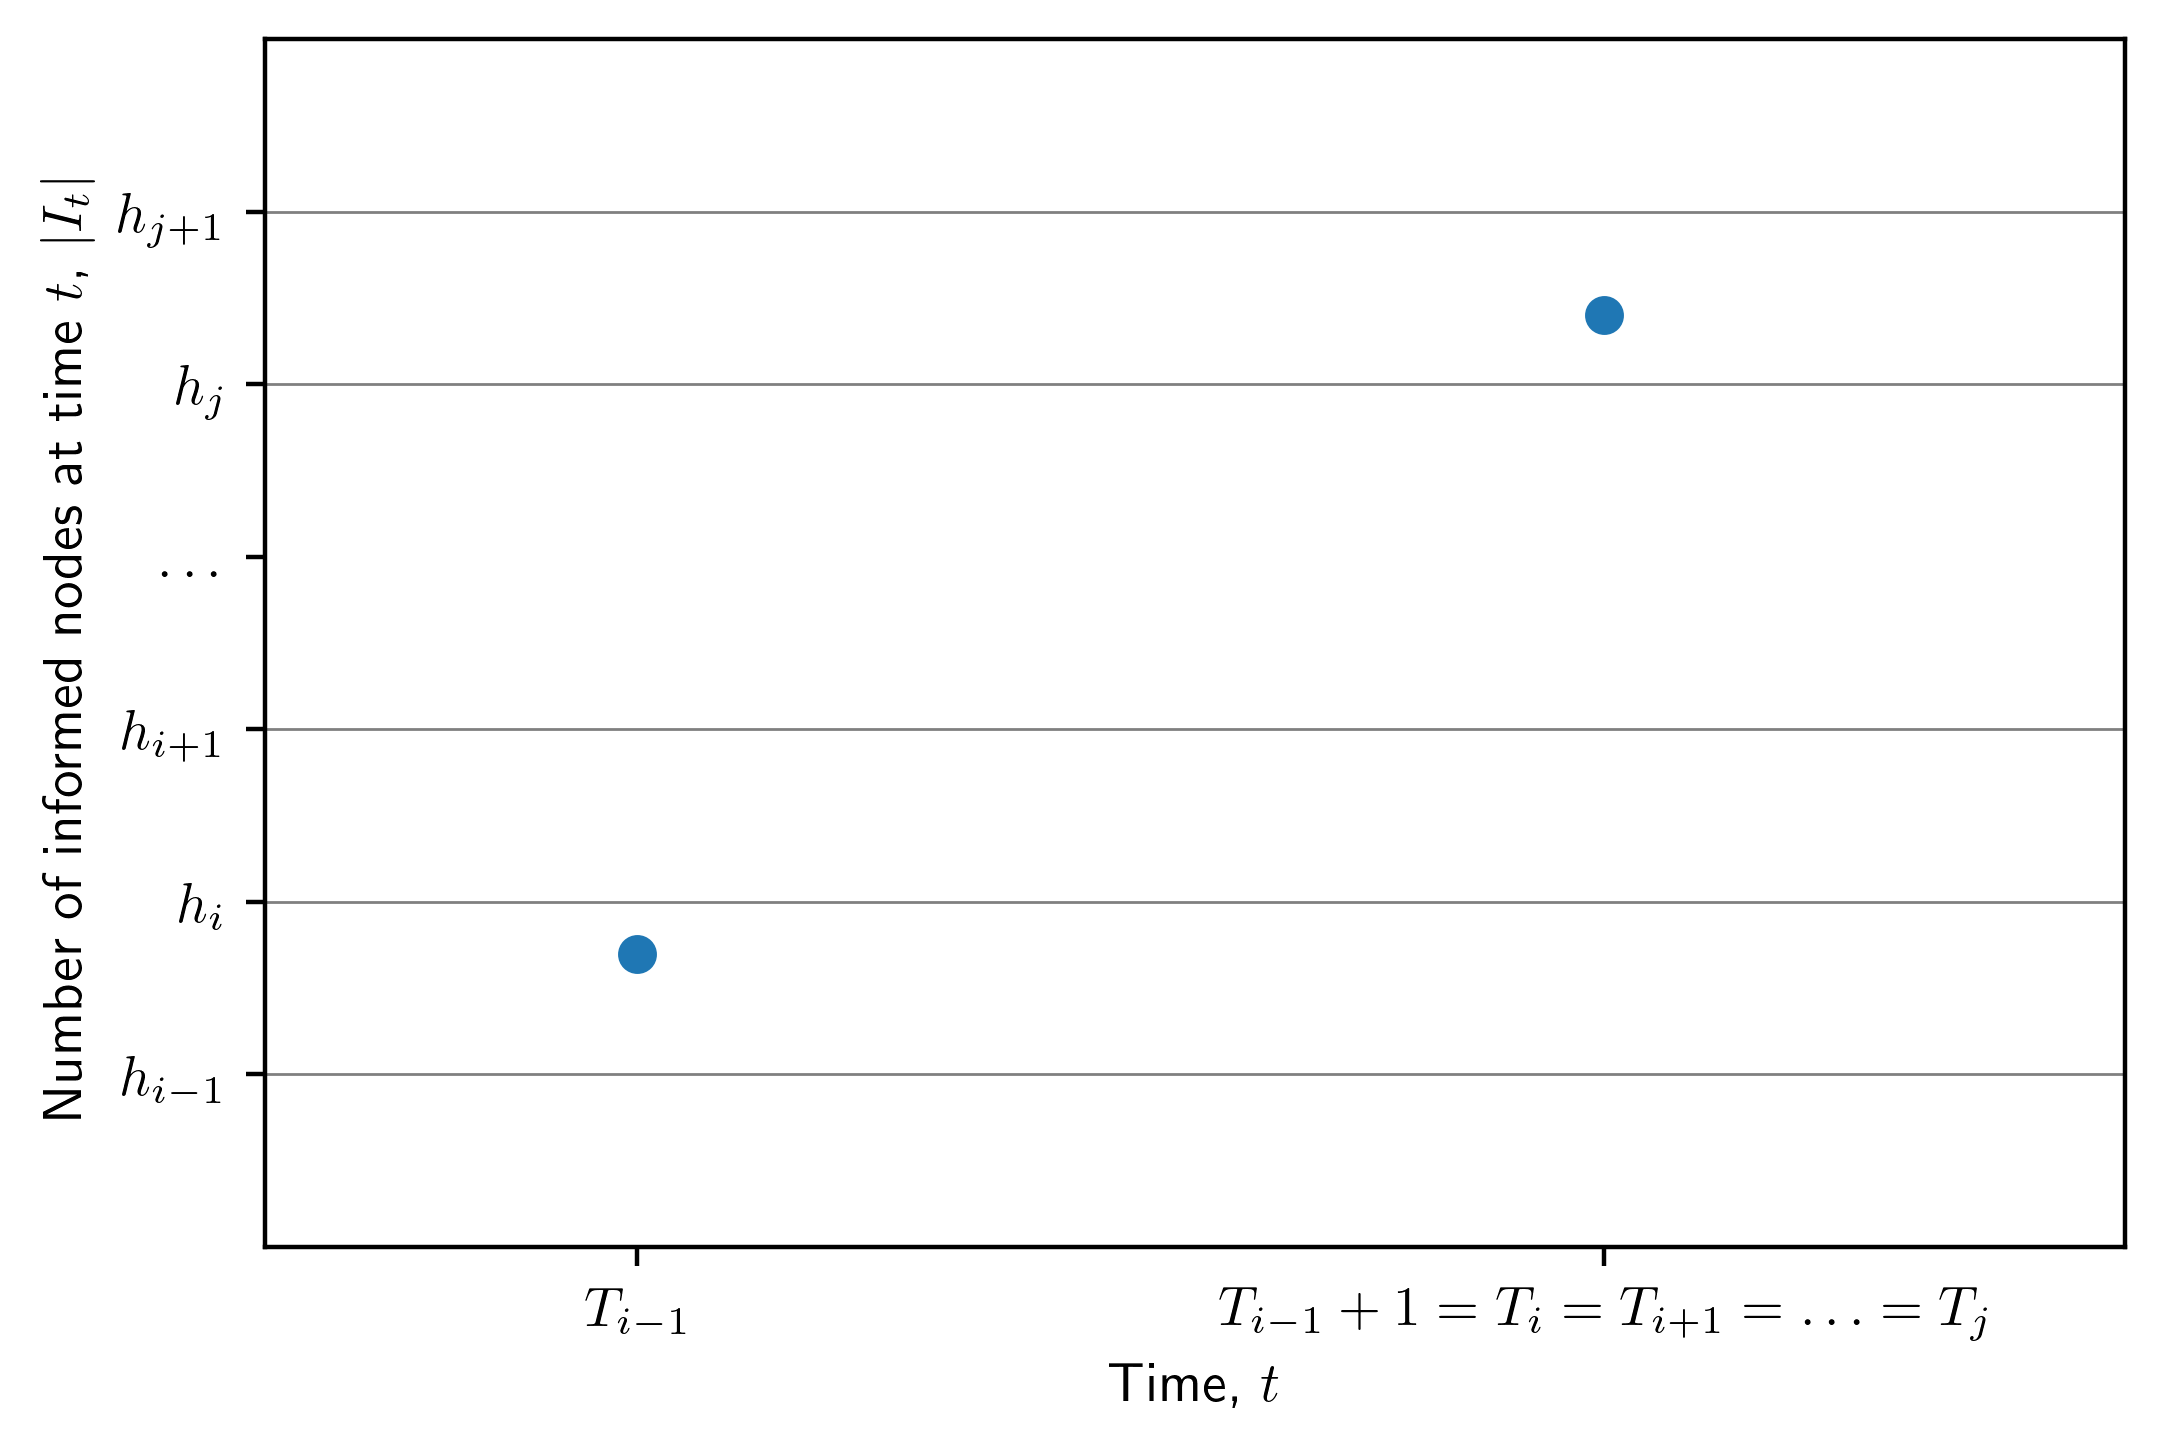
\includegraphics[width=1\textwidth]{./figures/flooding_jump.png}
		\caption{Behaviour of the number of informed nodes in the "jump" case}
		\label{fig:floodingJump}
	\end{figure}
	In this case the total time that has passed between $T_{i-1}$ and $T_j$ is 1, so we instead bound the whole jump interval as follows:
	
	% TODO: j doesn't exist case
	Let $j$ be the index such that $h_j < (1+k_i)h_{i-1} \leq h_{j+1}$, i.e. the last $j \geq i$ when $T_j = T_{i-1} + 1$, as in Figure \ref{fig:floodingJump}. % TODO: Check this equivalence - think it does hold
	% TODO: Figure here to illusttrate T_j, 
	% TODO: "may be the same as before" - what does this mean??? 
	Hence, by the definition of $j$, h
	\begin{align*}
		T_j - T_{i-1} &=1 \\ 
		&\leq \frac{\log (h_{j+1}) - \log(h_{i-1})}{\log(1+k_i) } \\
		& =\sum_{l=i}^{j+1} \frac{\log (h_{l}) - \log(h_{l-1})}{\log(1+k_i) } & \text{since the numerator forms a telescoping sum} \\
		& \leq \sum_{l=i}^{j+1} \frac{\log (h_{l}/h_{l-1})}{\log(1+k_l) } & \text{since } k_i \geq k_l \text{ for all } l \geq i \\
		& = \mathcal{O}\left(\sum_{l=i}^j \frac{\log (h_{l}/h_{l-1})}{\log(1+k_l) }\right)
 	\end{align*}

	We now use this equality to bound the growth of $T_s$, the first time at which more than $h_s = \frac{n}{2}$ nodes are aware of the rumour. We can express $T_s$ as a telescoping sum of intervals as follows:
	$$
		T_s = \sum_{i=2}^s T_i - T_{i-1}
	$$
	% TODO: T_1 = 0 is this consistent??
	For the $i^\text{th}$ interval, if $\frac{\log (h_i/h_{i-1})}{\log(1+k_i)} \geq 1$, we can apply the result from Case 1. If $\frac{\log (h_i/h_{i-1})}{\log(1+k_i)} < 1$, we apply Case 2 to bound the whole jump interval $[T_{i-1}, T_j]$, and continue the summation from $T_j$. % TODO: CHeck, problems from j+1 on case 2 result?
	Thus, $T_s$ can be bounded above by
	\begin{equation}\label{eq:floodingBoundExpression}
		\mathcal{O}\left(\sum_{i=1}^s \frac{\log \frac{h_i}{h_{i-1}}}{\log(1+k_i)}\right)
	\end{equation}
	Recall that $T_s$ is the first time that the number of informed nodes exceeds $h_s = \frac{n}{2}$. We now bound the time it takes until all nodes are aware of the rumour (which we denote $T_\text{all}$) from $T_s$.

	We argue that the length of the interval $[T_s, T_\text{all}]$ is also bounded by equation \ref{eq:floodingBoundExpression} using symmetry. Consider the set of uninformed nodes a time $t$, $U_t$. Note that if some node in $B(U_t)$ was aware of rumour in the previous time step, we would have a contradiction, since a node in $U_t$ would have been made aware of the rumour in round $t$ following Algorithm \ref{SyncFloodingAlgorithm}.
	Thus, at the end of the previous time step, none of nodes in $B(U_t)$ can have been aware of the rumour.
	Hence, at time $t-1$, $(U_t \cup B(U_t)) \subseteq U_{t-1}$, so $|U_t| + |B(U_t)| \leq |U_{t-1}|$.
	
	Let $i \leq s$ be the index such that $h_{i-1}< |U_t| \leq h_i$. Then since $G_t$ is an $(h_i, k_i)$-expander, 
	\begin{equation} \label{eq:floodingReverseBound}
		|U_{t-1}| \geq (1 + k_i)|U_t|
	\end{equation}
	Suppose we observe the rumour spreading process in reverse, starting at time $T_\text{all} - 1$ and finishing at the first time there are at least $\frac{n}{2}$ uninformed nodes (from the reverse perspective). We notice from equation \ref{eq:floodingReverseBound} that the growth in the number of uninformed nodes when watching the spreading process in reverse is subject to the same conditions as the growth in the number of informed nodes when watching the process forwards. Thus, by symmetry, the length of the interval $[T_s, T_\text{all}]$ can also be bounded by expression \ref{eq:floodingBoundExpression} in exactly the same way as the interval $[T_0, T_s]$. Hence, the spreading time $T_\text{all}$ is at most
	$$
		\mathcal{O}\left(\sum_{i=1}^s \frac{\log \frac{h_i}{h_{i-1}}}{\log(1+k_i)}\right)
	$$
	% TODO : Think about the stralling -1, T_0 vs T_1, need to bound [T_0, T_all]
\end{proof}

\section{Review of Discrete-time Markov Chains}

In this section we give a brief review of Markov chains and associated results needed for Section \ref{section:MEDNBound}. We assume that the reader is familiar with finite Discrete-time Markov chains, so omit the proofs in this section. For a full treatment of the subject see \cite{grimmetBook}.

% TODO: Make sure all motivated by intuition at least, specify definitions to establish conventions/terminology more than educate

% TODO: ROUGH - not told how converges, but should define "distribution of its current state after $n$ time steps", rely on intuituion

\section{Flooding on Markovian Evolving Dynamic Networks}\label{section:MEDNBound}

Until now, all the dynamic networks we have studied have been deterministic, in the sense that the evolution of topologies has been fixed. However, knowing the future topologies of the network may be unrealistic in practice. For example, when considering rumour spread on a real-world network such as the internet, we cannot say with certainty what connections will be present on a given time in the future. This motivates a generalistion of the dynamic network model where the sequence of topologies is drawn from some distribution. This distribution expresses our uncertainty in the future topologies of the network, but allows us to encode information about how we predict the shape of the network may evolve. Under this model, the dynamic network itself is a stochastic process, and a source of randomness. In this section, we analyse the rumour spreading time when a Markov chain is used to  generate the random sequence of topologies.

First we introduce a variation of the original Dynamic Network definition.

\begin{definition}
	Markovian Evolving Dynamic Network (MEDN)

	\noindent 
	Let $\mathcal{A}(V)$ be the set of all possible graphs on the vertex set $V$.
	A Markovian Evolving Dynamic Network is a random sequence of graphs $\mathcal{M} = (G_t)_{t \in \mathbb{N}}$ indexed by an integer time $t$, such that $\mathcal{G}$ is a Markov chain with state space $\mathcal{A}(V)$.
\end{definition}

We see that this definition adheres to the previous restriction that all topologies have the same vertex set. Since the network is Markovian, the distribution from which the next topology is draw depends only on the previous topology.

We say that a given MEDN $\mathcal{M}$ is stationary if the distribution of $G_0$ is a stationary distribution of $\mathcal{M}$. By the definition of a stationary distribution, in such an MEDN the probability that $G_t = G'$ for a given $G'$ is the probability that $G_t = G'$ under the stationary distribution, for any time step $t$. Hence, once the Markov chain associated with the network has reached equilibrium, % TODO: define "equalibrium"
the future evolution of the network effectively proceeds by independently sampling a topology from the stationary distribution at each time step. % TODO: Check if independent, get rid of "effectively"?

Under certain conditions, Markov chains converge to their stationary distributions. Thus, for the rest of this section we assume that our MEDNs have been running for a long enough such that when we inject the rumour the network is already in equilibrium. In this paper we don't discuss the conditions which allow for converge to the stationary distribution or how long the convergence takes, and assume that round 0 begins when we inject the rumour.
% TODO: What about if we started not in the stationary distributuion?? Further exploration needed. Or close to stationary? 

We now adapt the deterministic bound proved in Theorem \ref{theorem:DeterministicFloodingBound} to a MEDN, by adding details to proof from \cite{syncPaper}

% TODO: Is this a non-theorm? What does it acutally mean?

\begin{theorem}\label{theorem:markovSyncBound}
	Let $\mathcal{M} = (G_t)_{t \in \mathbb{N}}$  be a stationary Markovian evolving graph. Suppose also that there exists an increasing sequence $1 = h_0 \leq h_1 < \dots < h_s = \frac{n}{2}$ and decreasing sequence $k_1 \geq k_2 \geq \dots \geq k_s$ of positive real numbers, such that with probability $1-\frac{1}{n^2}$, the stationary distribution of $\mathcal{M}$ is a $(h_i, k_i)$-expander for every $i \in \{1, \dots , s\}$. Then the spreading time of $\mathcal{G}$ under algorithm \ref{SyncFloodingAlgorithm} is
	$$
		\mathcal{O}\left(\sum_{i=1}^s \frac{\log \frac{h_i}{h_{i-1}}}{\log(1+k_i)}\right)
	$$
	w.h.p.
\end{theorem}

Note that in previous bounds the source of randomness in the spreading time has been the rumour spreading algorithm, however in this bound the only source of randomness is the network itself.

We notice that in this theorem, instead of requiring every graph topology to satisfy the expansion conditions of Theorem \ref{theorem:DeterministicFloodingBound}, we only require that the same expansion properties hold w.h.p with respect to the stationary distribution. % TODO: REWORD??
Since each topology is sampled from the stationary distribution, these properties will hold for nearly all the topologies in the sequence. Thus, this theorem states that our deterministic bound will hold for MEDNs, as long as the long-term proportion of topologies in our network without strong expansion properties is bounded by $\frac{1}{n^2}$.

% TODO: Review this proof for order that makes sense, and check it actually holds

\begin{proof}
	For all $t \in \mathbb{N}$, let $A_t$ be the event that $G_t$ is an $(h_i, k_i)$-expander for all $1 \leq i \leq s$. Since $\mathcal{M}$ is stationary, we have that $\mathbb{P}(A_t) \geq 1 - \frac{1}{n^2}$ for all t. 

	Let $B$ denote the event we are interested in, namely that the rumour spreading time is 	
	$$
		\mathcal{O}\left(\sum_{i=1}^s \frac{\log \frac{h_i}{h_{i-1}}}{\log(1+k_i)}\right)
	$$

	Suppose that $A_k$ holds for all $k \leq n$. We claim that the rumour spreads in at most $n$ time steps with certainty. Since we have assumed that all topologies up to time $n$ are $(h_1, k_1)$-expanders, there are no isolated nodes, as such an isolated node $v$ would form a subset of size $1 \leq h_1$ with $B({v}) = 0 < k_1$, a contradiction. Thus, the network is connected for the first $n$ time steps. Hence, for any time step $t \leq n$ before all nodes are informed of the rumour, $B(I_t) \geq 1$, since there is only 1 connected component so $I_t$ must be connected  to $U_t$ by at least 1 edge. It follows that in each time step at least 1 new node becomes informed of the rumour by the operation of algorithm \ref{SyncFloodingAlgorithm}. Hence, at most $n$ steps are needed to spread the rumour when $A_k$ holds for all $k \leq n$. 

	Let $T$ denote the first time step at which all nodes are informed of the rumour. By Theorem \ref{theorem:DeterministicFloodingBound} we have that if $A_k$ holds for all $k \leq T$, then $T=\mathcal{O}\left(\sum_{i=1}^s \frac{\log (h_i/h_{i-1})}{\log(1+k_i)}\right)$, as once all the nodes have been informed, the expansion properties of the remaining topologies are irrelevant.

	Now we combine the previous two claims. By the first claim if $A_k$ holds for all $k \leq n$ we have that $T \leq n$, thus $A_k$ holds for all $k \leq T$. In this case, by the second claim we obtain that  $T=\mathcal{O}\left(\sum_{i=1}^s \frac{\log (h_i/h_{i-1})}{\log(1+k_i)}\right)$.

	Since we have shown that the event $\bigcap_{t=0}^n A_t \implies B$, we have that $\comp{B} \implies \comp{ \bigcap_{t=0}^n A_t} = \bigcup_{t=0}^n \comp{A_t}$. To finish the proof, we show that the event $\comp{B}$ occurs with vanishing probability, thus $B$ occurs w.h.p.

	\begin{align*}
		\mathbb{P}(\comp{B}) &\leq \mathbb{P}(\bigcup_{t=0}^n \comp{A_t}) & \text{by the inferred implication} \\ 
		& \leq n \mathbb{P}(\comp{A_t}) & \text{by the union bound}\\ 
		& \leq n \frac{1}{n^2} = \frac{1}{n} & \text{by the conditions on the stationary distribution}
	\end{align*}

	% TODO: THINK ABOUT h_0

\end{proof}

\section{Applying the bound to the Edge Markovian MEDN}\label{section:floodingBoundEdgeMarkovian}

In this section, we apply the bound proved in Theorem \ref{theorem:markovSyncBound} to a specific MEDN called the Edge-Markovian Network. We will also evaluate the quality of the bound by proving a lower bound on the spreading time, and comparing the results with simulations. 

First, we introduce and motivate the model.
\begin{definition}
	Edge-Markovian Network $\mathcal{M}(n, p, q)$

	\noindent
	Let $V$ be a vertex set, and $E = \left\{e : e \subseteq V, |e| = 2 \right\}$ be the set of all possible edges between vertices in $V$. 
	Let $\left\{\{X_e(t)\}_{t \in \mathbb{N}} : e \in E \right\}$ be a set of independent Markov chains on the state space $\{0,1\}$, each with the transition matrix
	\begin{center}
		\begin{tabular}{ c | c c }
		   & 0     & 1 \\ 
		\hline
		 0 & $1 - p$ & $p$ \\  
		 1 & $q$     & $1 - q$  
		\end{tabular}
	\end{center}
	An Edge-Markovian Evolving Network $\mathcal{M}(n, p, q) = \left\{(V, E_t) : t \in \mathbb{N} \right\}$ is a random sequence of graphs on the vertex set $V$ where $E_t = \left\{ e \in E : X_e(t) = 1 \right\}$, i.e. each edge $e$ is only present in the time steps when its associated Markov chain $X_e$ is in state 1.
\end{definition}
The Edge-Markovian Network models the situation when connections between nodes independently fail or are restored. The "birth" and "death" of each edge $e$ is dictated by its associated Markov chain $X_e$, where in each round, a present edge has probability $q$ of failing, and a missing edge has probability $p$ of restoration. Hence, for any given edge, after a geometrically distributed time with parameter $q$, a failure occurs. Restoring the edge takes a geometrically distributed time with parameter $p$ % TODO: WHAT DO FAILING AND RESTORATION MEAN

Since the future state of each edge is only dependent on current state, this Network is appropriate for modelling memoryless Networks where we can assume each edge acts independently with identical dynamics to other edges. For example, in a computer network we could imagine each  connection is randomly disrupted by an issue with probability $q$, and the affected connection is fixed with probability $p$ in each of the subsequent time steps. 

Now we will see that the set of Markov chains associated with the edges induces a Markov chain over the set of possible graphs on $V$, thus the Edge-Markovian Network is an MEDN.

% TODO: REPAIR-DELAY NETWORKS - any edge could fail, takes a few steps to fix, how to model, what is the stationary distribution?

\begin{lemma}
	The Edge-Markovian Network is a MEDN
\end{lemma}

\begin{proof}
	Since all the edges are memoryless, the distribution of which edges will be present in the subsequent round is only dependent on which edges are present currently. %TODO: Reword this
	Thus, the distribution over possible topologies in the following round is only dependent on the topology in the current round.
	Hence, the sequence of topologies is a Markov chain, so the network is an MEDN.
	% TODO: Include transition probabilities
\end{proof}

Since the Edge-Markovian Network is an MEDN, we can apply Theorem \ref{theorem:markovSyncBound} to bound the spreading time of Algorithm \ref{SyncFloodingAlgorithm}. Before applying the bound, we need to establish the stationary distribution of this network. First we establish when a stationary distribution exists for the Edge-Markovian MEDN.

\begin{lemma}
	An Edge-Markovian MEDN $\mathcal{M}(n, p, q)$ converges to a unique stationary distribution if $0 < p, q < 1$.
\end{lemma}

\begin{proof}
	If either $p=0$ or $q=0$, then the edges could get stuck in a present or not-present state, but if $0 < p, q$ then the Markov chain can always move to a new state. When we also have that $p, q < 1$, any set of edge insertions and deletions from an arbitrary state has non-zero probability. Thus, under these conditions, it is possible to transition between any two states in a single time step. Hence, the Markov chain is irreducible when $0 < p, q < 1$, so by Theorem \ref{theorem:uniqueStationaryDistribution}, a unique stationary distribution exists.

	If $p=q=1$, then the Markov chain is periodic as edges alternate between present and non-present each time step. However, if $p, q < 1$ no such periodic behaviour can take place with certainty, so the Markov chain is aperiodic.

	Hence, if $0 < p, q < 1$ the Markov chain is irreducible and aperiodic, thus by Theorem \ref{theorem:markovChainConvergence}
	it converges to a unique stationary distribution.
\end{proof}

For convenience, we assume that $0 < p, q < 1$ for the remainder of this section. Now we introduce the unique stationary distribution for the Edge-Markovian MEDN. 

\begin{definition}
	Erdős-Rényi Random Graph $G(n,\tilde{p})$

	\noindent	
	The Erdős-Rényi (ER) Random Graph is a distribution over all the possible graphs on a vertex set of size $n$, where each edge is present with probability $\tilde{p}$.
\end{definition}

Now we prove that the ER distribution $G(n,\tilde{p})$ is the stationary distribution for the Edge-Markovian MEDN for a specific $\tilde{p}$.

\begin{lemma}
	The stationary distribution of $\mathcal{M}(n, p, q)$ is the Erdős-Rényi distribution $G(n, \frac{p}{p+q})$ 
\end{lemma}

\begin{proof}
	Let 
	$$
		\pi = \left(\frac{q}{p+q}, \frac{p}{p+q}\right)
	$$ 
	be a distribution over the starting states of $X_e$ for any $t \in \mathbb{N}, e \in E$, % TODO: E not defined here
	where the first component is the probability of starting in state 0, and the second component is the probability of starting in state 1. First we show that $\pi$ is the stationary distribution for all the edge Markov chains.

	Let $M$ be the transition matrix for any of the edge Markov chains. We calculate the distribution over $\{0,1\}$ after a single round starting in distribution $\pi$. Observe that
	$$
		\pi M =
		\begin{bmatrix}
			\frac{q}{p+q} & \frac{p}{p+q}
		\end{bmatrix}
		\begin{bmatrix}
			1 - p & p \\
			q & 1 - q 
		\end{bmatrix}
		= \begin{bmatrix}
			\frac{q}{p+q} & \frac{p}{p+q}
		\end{bmatrix}
		= \pi
	$$
	thus $\pi$ is the stationary distribution of any $X_e$.
	
	Now we formulate the stationary distribution of the topology Markov chain. Note that this is a distribution over possible topologies on the vertex set $V$. When all edges start in the stationary distribution, at any time step $t$, $X_e(t) = 1$ with probability $\frac{p}{p+q}$ by the stationarity of $\pi$. Hence, under this initial distribution, each edge is present with probability $\frac{p}{p+q}$ in any time step. Note that this distribution over the possible topologies is not dependent on the topology of the network at any other time, hence it is stationary. % TODO: IS this clear direction -> distribution is stationary

	We recognise this distribution as the $G(n, \frac{p}{p+q})$ ER Random Graph distribution.
\end{proof}

Thus, when we start the Markov chain in a topology chosen at random according to the $G(n, \frac{p}{p+q})$ distribution, the distribution of topologies for the next step is again the $G(n, \frac{p}{p+q})$ distribution. Inductively, the distribution of the topology of the network at any time step is $G(n, \frac{p}{p+q})$.

To apply Theorem \ref{theorem:markovSyncBound}, we need to compute expansion properties of the stationary distribution that hold w.h.p. We do this for an arbitrary $G(n, p)$ distribution.

\begin{lemma}\label{lemma:GnpExpansion}
	Let $p \geq c\frac{\log n}{n}$ for a sufficiently large constant $c$. For a $G(n, p)$ graph we have that for all $S \subseteq V$ such that $|S| \leq \frac{n}{2}$
	$$
		|B(S)| \geq \frac{n}{c} \min \left\{ |S|p, 1 \right\} 
	$$
	with probability at least $1 - \frac{1}{n^2}$, for large $n$. 
\end{lemma}

% TODO: mention OMit proof citing elementary probability + not relevant

Lemma \ref{lemma:GnpExpansion} tells us that if we choose a random topology according to the $G(n, p)$ distribution with a suitably large $p$, w.h.p the boundaries of all "small" sets are large. Note that the condition on $p$ scales with the number of nodes $n$. % TODO: Expanding

In Lemma \ref{lemma:GnpExpander}, we use Lemma \ref{lemma:GnpExpansion}, to establish expansion properties for the $G(n,p)$ distribution.

% TODO: Interpretation of lemma in terms of expander graphs

\begin{lemma}\label{lemma:GnpExpander}
	Let $p \geq c\frac{\log n}{n}$ for a sufficiently large constant $c$, and large $n$. With probability at least $1- n^2$, a topology $G$ drawn from the $G(n, p)$ distribution is a $(h, p\frac{n}{c})$-expander for all $1 \leq h \leq \frac{1}{p}$ and a $(h, \frac{1}{h}\frac{n}{c})$-expander for all $\frac{1}{p} \leq h \leq \frac{n}{2}$
\end{lemma}

\begin{proof}
	Suppose 
	\begin{equation}\label{eq:GnpExpansionBound}
		|B(S)| \geq \frac{n}{c} \min \left\{ h p, 1 \right\} 
	\end{equation}
	holds for all $S$ such that $1 \leq |S| \leq \frac{n}{2}$. 
	Let $1 \leq h \leq \frac{n}{2}$. We consider 2 cases. 

	\textbf{Case 1.} $1 \leq h \leq \frac{1}{p}$. 

	Consider an arbitrary subset $S$ such that $h' = |S| \leq h$.
	By equation \ref{eq:GnpExpansionBound}, 
	$$
		|B(S)| \geq \frac{n}{c} \min \left\{ h' p, 1 \right\} = \frac{n}{c}h'p = p\frac{n}{c} |S|
	$$
	thus $G$ is a $(h, p\frac{n}{c})$-expander.
	Consider an arbitrary subset $S$ such that $h' = |S| \leq h$. 

	\textbf{Case 2.} $\frac{1}{p} \leq h \leq \frac{n}{2}$

	Consider an arbitrary subset $S$ such that $h' = |S| \leq h$.

	\textbf{Case 2a.}
	Suppose $1 \leq h' \leq \frac{1}{p}$. 
	
	Similarly to Case 1, 
	$$
		|B(S)| \geq p\frac{n}{c} |S|
	$$
	Since $h \geq \frac{1}{p}$, we observe that 
	$$
		|B(S)| \geq \frac{1}{h}  \frac{n}{c} |S|
	$$ 

	\textbf{Case 2b.} Suppose $\frac{1}{p} \leq h' \leq \frac{n}{2}$
	By equation \ref{eq:GnpExpansionBound}, 
	$$
		|B(S)| 
		\geq \frac{n}{c} \min \left\{ h' p, 1 \right\} 
		= \frac{n}{c}\frac{|S|}{h'} 
		\geq \frac{1}{h} \frac{n}{c}|S|
	$$

	Hence, $G$ is a $(h, \frac{1}{h} \frac{n}{c})$-expander.

	By Lemma \ref{lemma:GnpExpansion}, equation \ref{eq:GnpExpansionBound} holds with probability at least $1 - \frac{1}{n^2}$, hence the expansion properties also hold with probability at least $1 - \frac{1}{n^2}$.
\end{proof}

Now we apply Theorem \ref{theorem:markovSyncBound} to the Edge-Markovian Dynamic Network.

\begin{theorem}\label{theorem:edgeMarkovianFloodingBound}
	Let $\mathcal{M}(n, p, q)$ be a stationary Edge-Markovian Dynamic Network. If $\hat{p} = \frac{p}{p+q} \geq c \frac{\log n}{n}$ for a sufficiently large $c$ then w.h.p, the spreading time of Algorithm \ref{SyncFloodingAlgorithm} in $\mathcal{M}(n, p, q)$ is at most
	$$
		\mathcal{O}\left(\frac{\log n}{\log n\hat{p}} + \log \log n\hat{p} \right)
	$$
\end{theorem}

We take a moment to consider the role of $\hat{p}$. Note that $p$ and $q$ may be functions of $n$. However, since both quantities are constants once $n$ has been fixed, we omit function notation for brevity.

In the context of the Edge-Markovian model, the larger the ratio $\frac{p}{p+q}$, the less often edges fail, and the faster edges recover. %TODO: Could be misinterpreted
This in turn improves the likelihood that each topology contains many edges, increasing the speed at which the rumour spreads. This intuition is reflected in the bound given by Theorem \ref{theorem:edgeMarkovianFloodingBound}: the closer $\hat{p}$ is to 1, the smaller the $\frac{\log n}{\log n \hat{p}}$ term will be. However, interestingly the $\log \log n \hat{p}$ term increases with $\hat{p}$, which goes against our intuition, as this term will be larger for denser graphs. 
This indicates that our bound may not always be tight, which we will explore in Section \ref{section:edgeMarkovianFloodingBoundEvaluation}. % TODO: IS THIS TRUE?


\begin{proof}
	Let $\hat{p}$ denote $\frac{p}{p+q}$. 
	By Lemma \ref{lemma:GnpExpansion}, the stationary distribution of $\mathcal{M}(n, p, q)$ is an $(i, k_i)$-expander for $1 \leq i \leq \frac{n}{2}$ where 
	\begin{equation*}
		k_i = 
		\begin{cases*}
			\frac{n\hat{p}}{c} & $1 \leq i \leq \floor{\frac{1}{\hat{p}}}$ \\
			\frac{n}{ci} & $\floor{\frac{1}{\hat{p}}} \leq i \leq \frac{n}{2}$
		\end{cases*}
	\end{equation*}
	By Theorem \ref{theorem:DeterministicFloodingBound} we have that the spreading time is at most
	$$
		\mathcal{O}\left(\sum_{i=1}^\frac{n}{2} \frac{\log \frac{i}{\max\{i-1,1\}}}{\log(1+k_i)}\right)
	$$
	w.h.p.
	Since $\log \frac{i}{i-1} \leq \frac{1}{i}$ for $i \geq 2$, % TODO: Justify
	this quantity is bounded above by 
	$$
		\mathcal{O}\left(\sum_{i=1}^\frac{n}{2} \frac{1}{i\log(1+k_i)}\right)
	$$
	By substituting for $k_i$ in the summation, we have the that the order of the spreading time is bounded w.h.p by
	$$
		\sum_{i=1}^{\floor{1/\hat{p}}} \frac{1}{i\log(1+\frac{n\hat{p}}{c})} 
		+
		\sum_{i=\floor{1/\hat{p}} + 1}^\frac{n}{2} \frac{1}{i\log(1+\frac{n}{ci})} 
	$$
	We bound each of the sums separately.

	\textbf{First Sum.}

	Using that $\sum_{i=1}^m 1/i \leq \log m + 1$, %TODO: Justify
	we observe that
	$$
		\frac{1}{\log(1+\frac{n\hat{p}}{c})} \sum_{i=1}^{\floor{1/\hat{p}}} \frac{1}{i} 
		\leq 
		\frac{\log \frac{1}{\hat{p}} + 1}{\log(1+\frac{n\hat{p}}{c})} 
		= 
		\mathcal{O}\left(\frac{\log n}{\log(n\hat{p})}\right)
	$$
	where the final equality holds since $\hat{p} \geq \frac{c \log n}{\log n}$

	\textbf{Second Sum.}

	We split the second sum again into
	$$	
		\sum_{i=\floor{1/\hat{p}} + 1}^{\ceil{n/c}-1} \frac{1}{i\log(1+\frac{n}{ci})} 
		+ 
		\sum_{i=\ceil{n/c}}^\frac{n}{2} \frac{1}{i\log(1+\frac{n}{ci})} 
	$$
	Note that
	\begin{align*}
		\sum_{i=\floor{1/\hat{p}} + 1}^{\ceil{n/c}-1} \frac{1}{i\log(1+\frac{n}{ci})} 
		& \leq \sum_{i=\floor{1/\hat{p}} + 1}^{\ceil{n/c}-1} \frac{1}{i\log(\frac{n}{ci})} \\
		& \leq \int_{\floor{1/\hat{p}}}^{\ceil{n/c}-1} \frac{1}{x\log(1+\frac{n}{cx})} dx \\
		\intertext{since $f(x) = x\log(1+\frac{n}{cx})$ is non-negative and concave on the interval $[\floor{1/\hat{p}}, \ceil{n/c}]$ }
		& = \left[-\log\log \frac{n}{cx}\right]_{\floor{1/\hat{p}}}^{\ceil{n/c}-1} \\
		&= \mathcal{O}(\log \log (n \hat{p}))
	\end{align*}
	Since $\log(1+x) \geq \frac{x}{1+x}$ for $x < 1$ we observe that
	\begin{align*}
		\sum_{i=\ceil{n/c}}^\frac{n}{2} \frac{1}{i\log(1+\frac{n}{ci})} 
		& \leq 
		\sum_{i=\ceil{n/c}}^\frac{n}{2} \frac{(1 + \frac{n}{ci})}{i\frac{n}{ci}} 
		= 
		\sum_{i=\ceil{n/c}}^\frac{n}{2} \left( \frac{c}{n} + \frac{1}{i} \right) \\
		& \leq 
		\sum_{i=\ceil{n/c}}^\frac{n}{2} \left( \frac{c}{n} + \frac{c}{n} \right)
		= \mathcal{O}(1)
	\end{align*}

	To obtain the result, we recombine the summations
	$$
		\mathcal{O}\left(\sum_{i=1}^\frac{n}{2} \frac{\log \frac{i}{\max\{i-1,1\}}}{\log(1+k_i)}\right) =
		\mathcal{O}\left(\frac{\log n}{\log (n\hat{p})} + \log \log (n\hat{p})\right)
	$$

\end{proof}

Theorem \ref{theorem:edgeMarkovianFloodingBound} holds if $\hat{p}$ is at least $c \frac{\log n}{n}$ for a sufficiently large constant $c$, but what happens if $\hat{p} = o(\frac{\log n}{n})$? % TODO: Is mixing little o and concrete inequalities confusing?
It turns out that in this case we are unable to apply Theorem \ref{theorem:markovSyncBound}, so the assumption that $\hat{p} \geq c \frac{\log n}{n}$ is necessary for the proof as well as sufficient.

For the $G(n, \hat{p})$ distribution, it is well known that if $\hat{p} = o(\frac{\log n}{n})$, then w.h.p the graph will be disconnected \cite{complexNetworksRandomGraphs}. Since the graph can be split into at least two connected components, we notice that the smaller component is a set of size at most $\frac{n}{2}$ with an empty boundary. Hence, w.h.p, the graph is not a $(\frac{n}{2}, k)$-expander for any positive $k$. This is a condition for Theorem \ref{theorem:markovSyncBound}, hence we cannot apply the bound in cases where $\hat{p} = o(\frac{\log n}{n})$.

Bounding the spreading time of the Edge-Markovian Network in cases where $\hat{p} = o(\frac{\log n}{n})$ could be an interesting area for further study. Each topology will be disconnected w.h.p, but unlike the static $G(n,p)$ graph, the changing edges allow the rumour to spread between sets of nodes which were previously disconnected, and eventually inform all nodes in the network.
% TODO: Define "w.h.p"

\section{Evaluating the quality of the bound}\label{section:edgeMarkovianFloodingBoundEvaluation}

% TODO: Note \hat{p} is a function of n
% lower bound on mixing time
% TODO: Why can't generalise to varying t? (Non-homogenous MC)

In this section we evaluate how tight the bound in Theorem \ref{theorem:edgeMarkovianFloodingBound} is, using lower bounds on the spreading time and simulations. % TODO: Rephrase 
We start with a lower bound on the spreading time of Algorithm \ref{SyncFloodingAlgorithm} on the stationary Edge-Markovian Network.

\begin{theorem}\label{theorem:edgeMarkovianLowerBound}
	Let $\mathcal{M}(n, p, q)$ be a stationary Edge-Markovian Dynamic Network. If $\hat{p} = \frac{p}{p+q} \geq c \frac{\log n}{n}$ for a sufficiently large $c$ then w.h.p, the spreading time of Algorithm \ref{SyncFloodingAlgorithm} in $\mathcal{M}(n, p, q)$ is at least 
	$$
		\Omega\left(\frac{\log n}{\log (n \hat{p})}\right)
	$$
\end{theorem}

\begin{proof}
	Let $\delta_{v,t}$ be the degree of node $v \in V$ at time $t$. Since each topology is distributed according to the ER $G(n, \hat{p})$ distribution, $\delta_{v,t} \sim \text{Binomial}(n-1,\hat{p})$, as each of the $n-1$ other nodes have probability $\hat{p}$ of sharing an edge with $v$ in $G_t$. Thus,
	\begin{align*}
		\mathbb{P}(\delta_{v,t} \geq 2n\hat{p}) 
		& \leq \mathbb{P}(\text{Binomial}(n, \hat{p}) \geq 2n\hat{p}) \\ 
		\intertext{since the $\text{Binomial}(n, \hat{p})$ distribution stochastically dominates the $\text{Binomial}(n-1, \hat{p})$ distribution} % TODO: Prove in chapter:Prelims and cite
		& \leq \exp(-\frac{n\hat{p}}{3}) \\
		\intertext{by the Chernoff bound. We omit the proof of the Chernoff bound for brevity, but refer the reader to \cite{binomialChernoff} for a full proof.} % TODO: Move earlier if used there
		& \leq \exp(-\frac{c \log n}{3}) = n^{-\frac{c}{3}}
		\intertext{since $\hat{p} \geq \frac{c \log n}{n}$}
	\end{align*}
	By taking $c=9$, we obtain $\mathbb{P}(\delta_{v,t} > 2n\hat{p}) \leq n^{-3}$.
	We use this result to bound the probability that for a given time $t$, there exists a node with degree at least $2n\hat{p}$.
	$$
		\mathbb{P}\left(\bigcup_{v \in V} \left\{ \delta_{v,t} \geq 2n\hat{p}\right\} \right) 
		\leq 
		\sum_{v \in V}
		\mathbb{P}(\delta_{v,t} \geq 2n\hat{p}) 
		=
		n \mathbb{P}(\delta_{v,t} \geq 2n\hat{p}) 
		\leq
		n^{-2} 
	$$
	Denote maximum degree of $G_t$ as $\Delta_t$. Thus, by the previous union bound, the probability that $\Delta_t$ is at least $2n\hat{p}$ is at most $n^{-2}$ for all $t$. Now we use another union bound to bound the probability that the maximum degree of the network is at least $2n\hat{p}$ at any time step in the first $n$ rounds. % TODO: Exceeds is wrong word.
	$$
		\mathbb{P}\left(\bigcup_{t \in [n]} \left\{ \Delta_t > 2n\hat{p}\right\} \right) 
		\leq 
		\sum_{t \in [n]}
		\mathbb{P}(\Delta_t \geq 2n\hat{p}) 
		=
		n \mathbb{P}(\Delta_t \geq 2n\hat{p}) 
		\leq
		\frac{1}{n}
	$$
	Hence, w.h.p, in the first $n$ time steps all nodes have degree less than $2n\hat{p}$.

	For the remainder of the proof, we assume the high probability scenario where all nodes have degree less than $2n\hat{p}$ for the first $n$ rounds.
	Observe that in the first $n$ rounds, each node can spread the rumour to at most $2n\hat{p} - 1$ other nodes, since it has at most $2n\hat{p} - 1$ neighbours.
	Thus, in round $t$ the number of newly informed nodes is at most $(2n\hat{p} - 1)|I_t|$, since each of the $|I_t|$ informed nodes can spread the rumour to at most $2n\hat{p} - 1$ uninformed nodes. Hence, by induction at time $t < n$ the number of informed nodes is at most $(2n\hat{p})^t$.

	\textbf{Base Case.} $t=0$.

	Initially only one node is aware of the rumour, so $|I_0| = 1 = (2n\hat{p})^0$, hence the claim holds in this case.

	\textbf{Inductive Case.} $t=k+1$.

	We assume that $|I_k| \leq (2n\hat{p})^k$. Then 
	$$
		|I_{k+1}| \leq |I_k| + (2n\hat{p} - 1)|I_k| = (2n\hat{p})|I_k| \leq (2n\hat{p})^{k+1}
	$$
	by the induction hypothesis, hence the claim holds in this case.

	Let $\tau = \frac{\log (n/2)}{\log(2n\hat{p})}$. Note that for sufficiently large $n$, $\tau < n$, since $\hat{p} \geq c \frac{\log n}{n}$.  %TODO: Check if this is true - what if \hat{p} grows slowly in n??
	Hence, we obtain that for all times $t < \tau = \frac{\log (n/2)}{\log(2n\hat{p})}$, the number of informed nodes is at most $\frac{n}{2}$. Thus, the spreading time is at least 
	$$
		\tau = \Omega\left(\frac{\log n}{\log(n \hat{p})}\right)
	$$
\end{proof}

Note that the lower bound on the spreading time is exactly the first term of the bound proved in Theorem \ref{theorem:edgeMarkovianFloodingBound}. Hence, when $\frac{\log n}{\log (n\hat{p})}$ is the dominant term, the bound is tight. In fact, under these circumstances, we characterise the exact scaling for the spreading time up to constants.

\begin{corollary}\label{corollary:edgeMarkovianThetaBound}
	Let $\mathcal{M}(n, p, q)$ be a stationary Edge-Markovian Network such that 
	$$
		c \frac{\log n}{n} \leq \hat{p} \leq  \frac{n^\frac{1}{\log \log n}}{n}
	$$
	for a sufficiently large $c$. Then, w.h.p, the spreading time of Algorithm \ref{SyncFloodingAlgorithm} on $\mathcal{M}(n, p , q)$ is 
	$$
		\Theta\left(\frac{\log n}{\log(n\hat{p})}\right)
	$$
	and the bound from Theorem \ref{theorem:markovSyncBound} is tight.
\end{corollary}

\begin{proof}
	Since $\hat{p} \geq c \frac{\log n}{n}$, w.h.p, the spreading time is at most 
	$$
		\mathcal{O}\left(\frac{\log n}{\log n\hat{p}} + \log \log n\hat{p} \right)
	$$ by Theorem \ref{theorem:edgeMarkovianFloodingBound}, and at least 
	$$
		\Omega\left(\frac{\log n}{\log(n \hat{p})}\right)
	$$
	by Theorem \ref{theorem:edgeMarkovianLowerBound}.
	Note that 
	$$
		\frac{\log n}{\log(n\hat{p})} \geq \frac{\log n}{\log(n^\frac{1}{\log \log n})} = \log \log n
	$$
	As $\hat{p} \geq 1$, $\log \log n \geq \log \log (n\hat{p})$, so the first term of the upper bound is dominant and w.h.p, the spreading time is at most 
	$$
		\mathcal{O}\left(\frac{\log n}{\log n\hat{p}}\right)
	$$
	Hence the spreading time is
	$$
		\Theta\left(\frac{\log n}{\log(n\hat{p})}\right)
	$$
	and the upper bound is tight.
\end{proof}

% TODO: BE explicit - bound is tight when phat in above range

% TODO: DEFINE WHP in chapter:Prelims
 
% TODO: simulations outside tight range p like ((logn)^k)/n

We verify this result with simulations.

\begin{figure}[h]
	\centering
	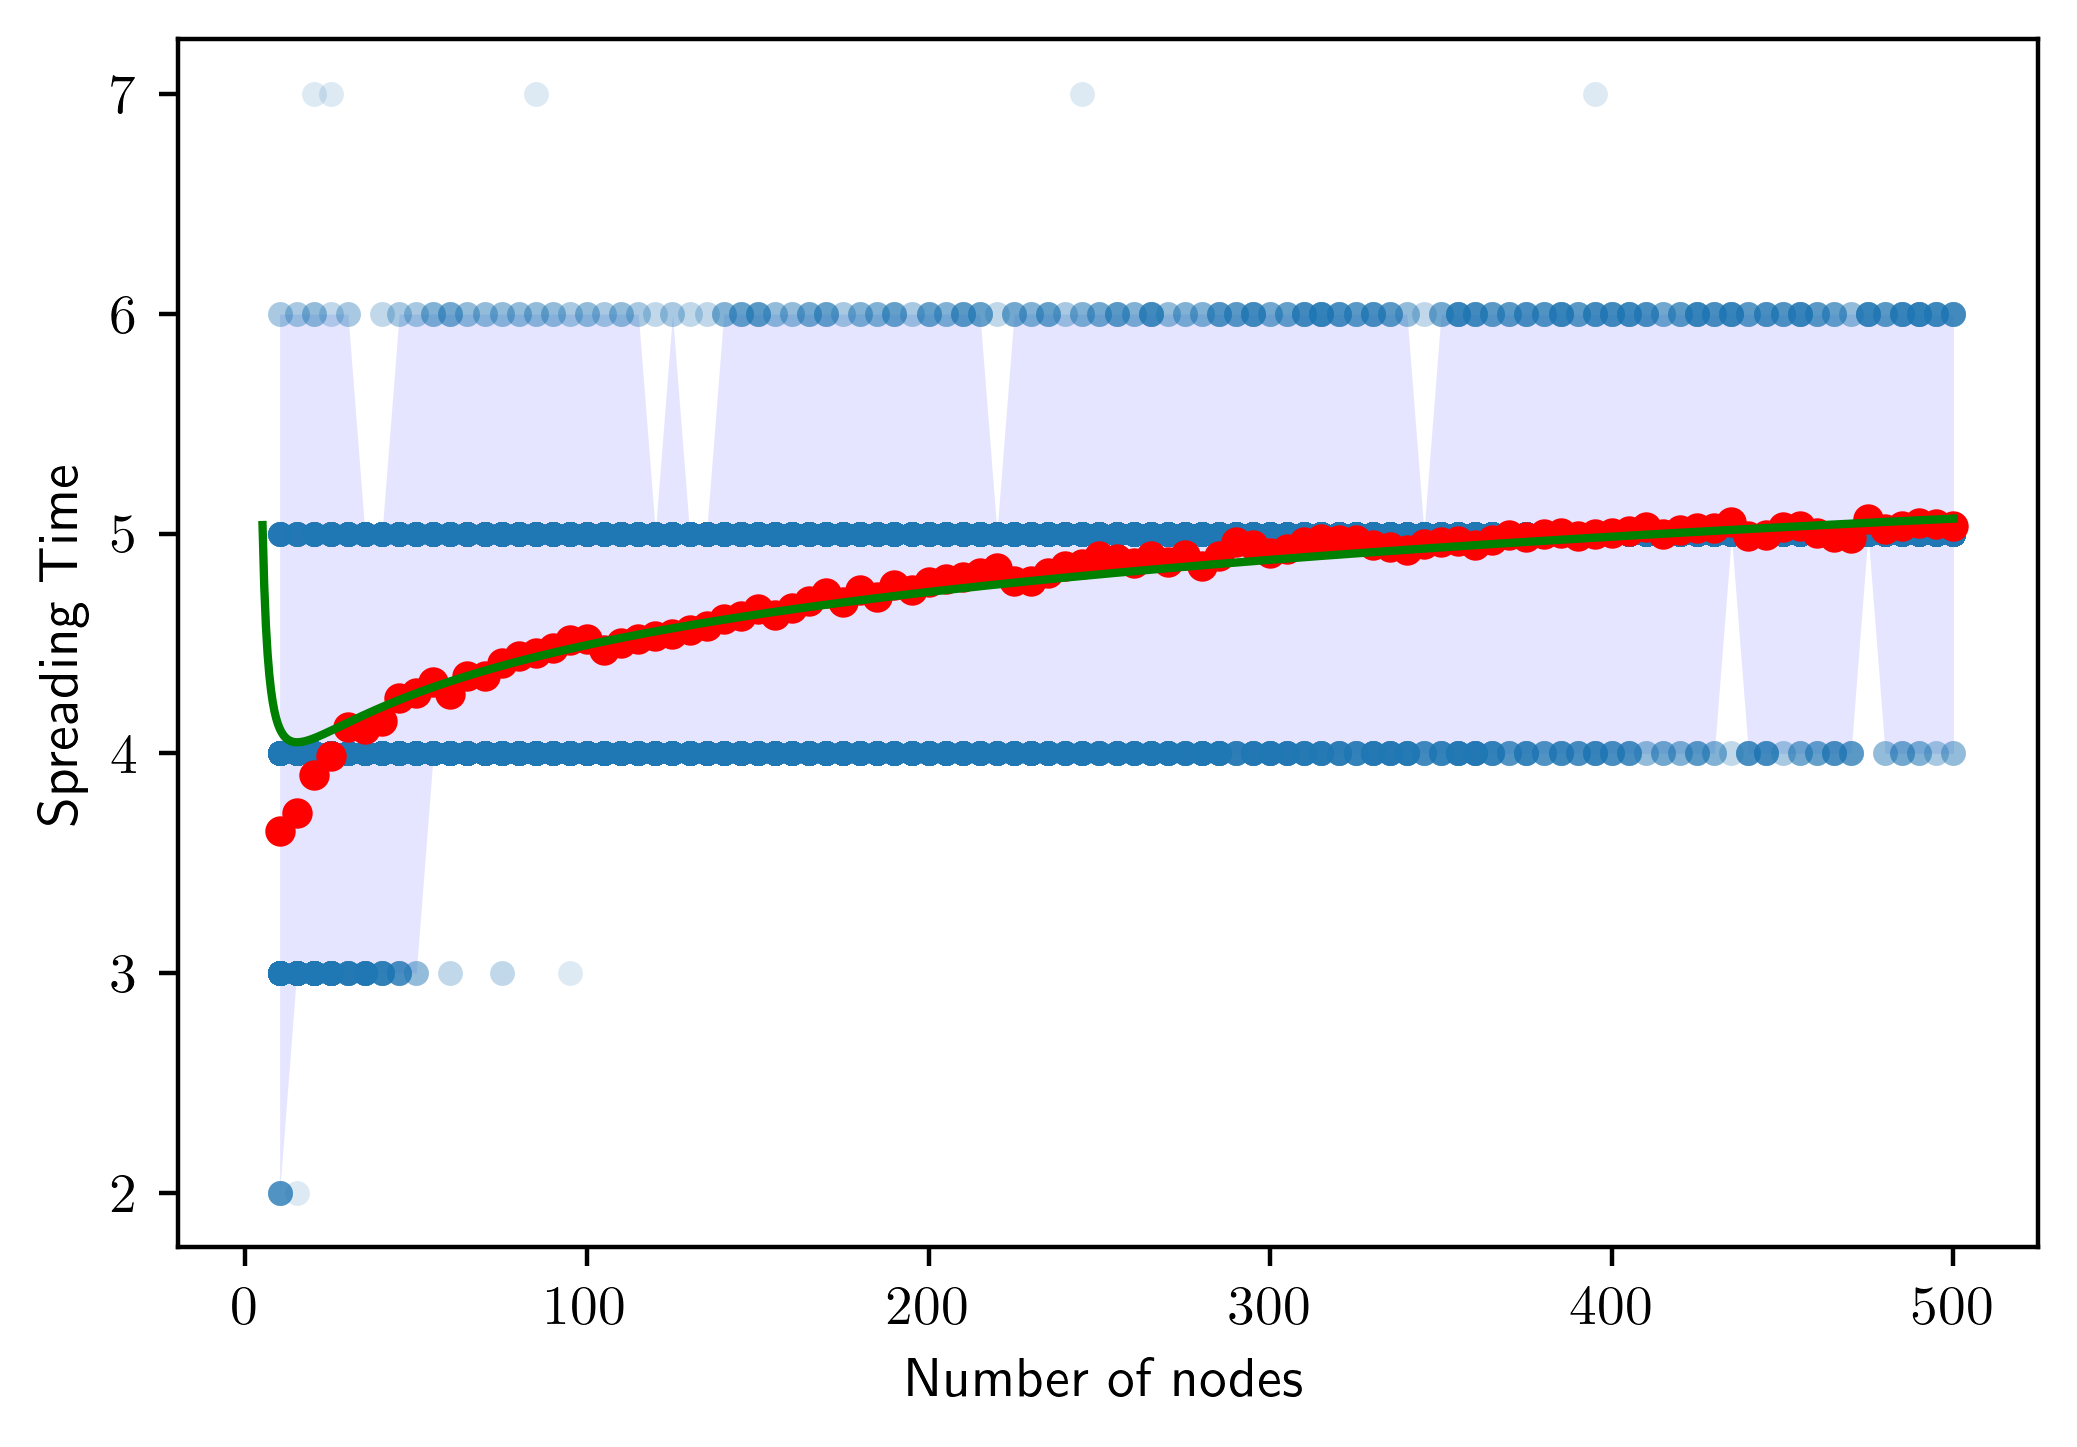
\includegraphics[width=1\textwidth]{./figures/flooding_simulation_min_p_with_error.png}
	\caption{Results of Edge-Markovian Dynamic Network spreading time simulations when $\hat{p} = \frac{\log n}{n}$}
	\label{fig:floodingGnpSimResultsTight}
\end{figure}

% TODO: BOTTOM OF INTERVAL
Figure \ref{fig:floodingGnpSimResultsTight} displays the simulation results for rumour spread on the stationary Edge-Markovian Network when $\hat{p} = \frac{\log n}{n}$.
Since the rumour spreads in discrete rounds, each of the simulation results (represented as a blue point) lies on an integer value. Each simulation was repeated 300 times for each network size, with the means displayed in red. In green, we have plotted the bound from Theorem \ref{theorem:edgeMarkovianFloodingBound}, i.e.
$$
	g(n) 
	= \Theta\left(\frac{\log n}{\log (n\hat{p})}\right) 
	= \Theta\left(\frac{\log n}{\log \log n}\right)
$$
The areas within the light blue section contains a $1-\frac{1}{n}$ fraction of the simulation results for each network size $n$. Observe that this region varies from the mean by $\mathcal{O}(1)$. Thus, we can reason about the w.h.p spreading time growth by comparing the bound to the average spreading time growth. 
% TODO: LIMITATION IN METHOD: DOES THE VARIANCE AROUND THE MEAN CHANGE??
As expected, for large $n$, the simulation times closely follow the bound once an appropriate scaling constant has been chosen. Note that for small $n \leq 50$, the expected spreading time does not match the simulated spreading times. However, this is not cause for concern as Corollary \ref{corollary:edgeMarkovianThetaBound} is only concerned with the asymptotic behaviour of the spreading times. % TODO: "Concerned" twice

% random variable, from network

\begin{figure}[h]
	\centering
	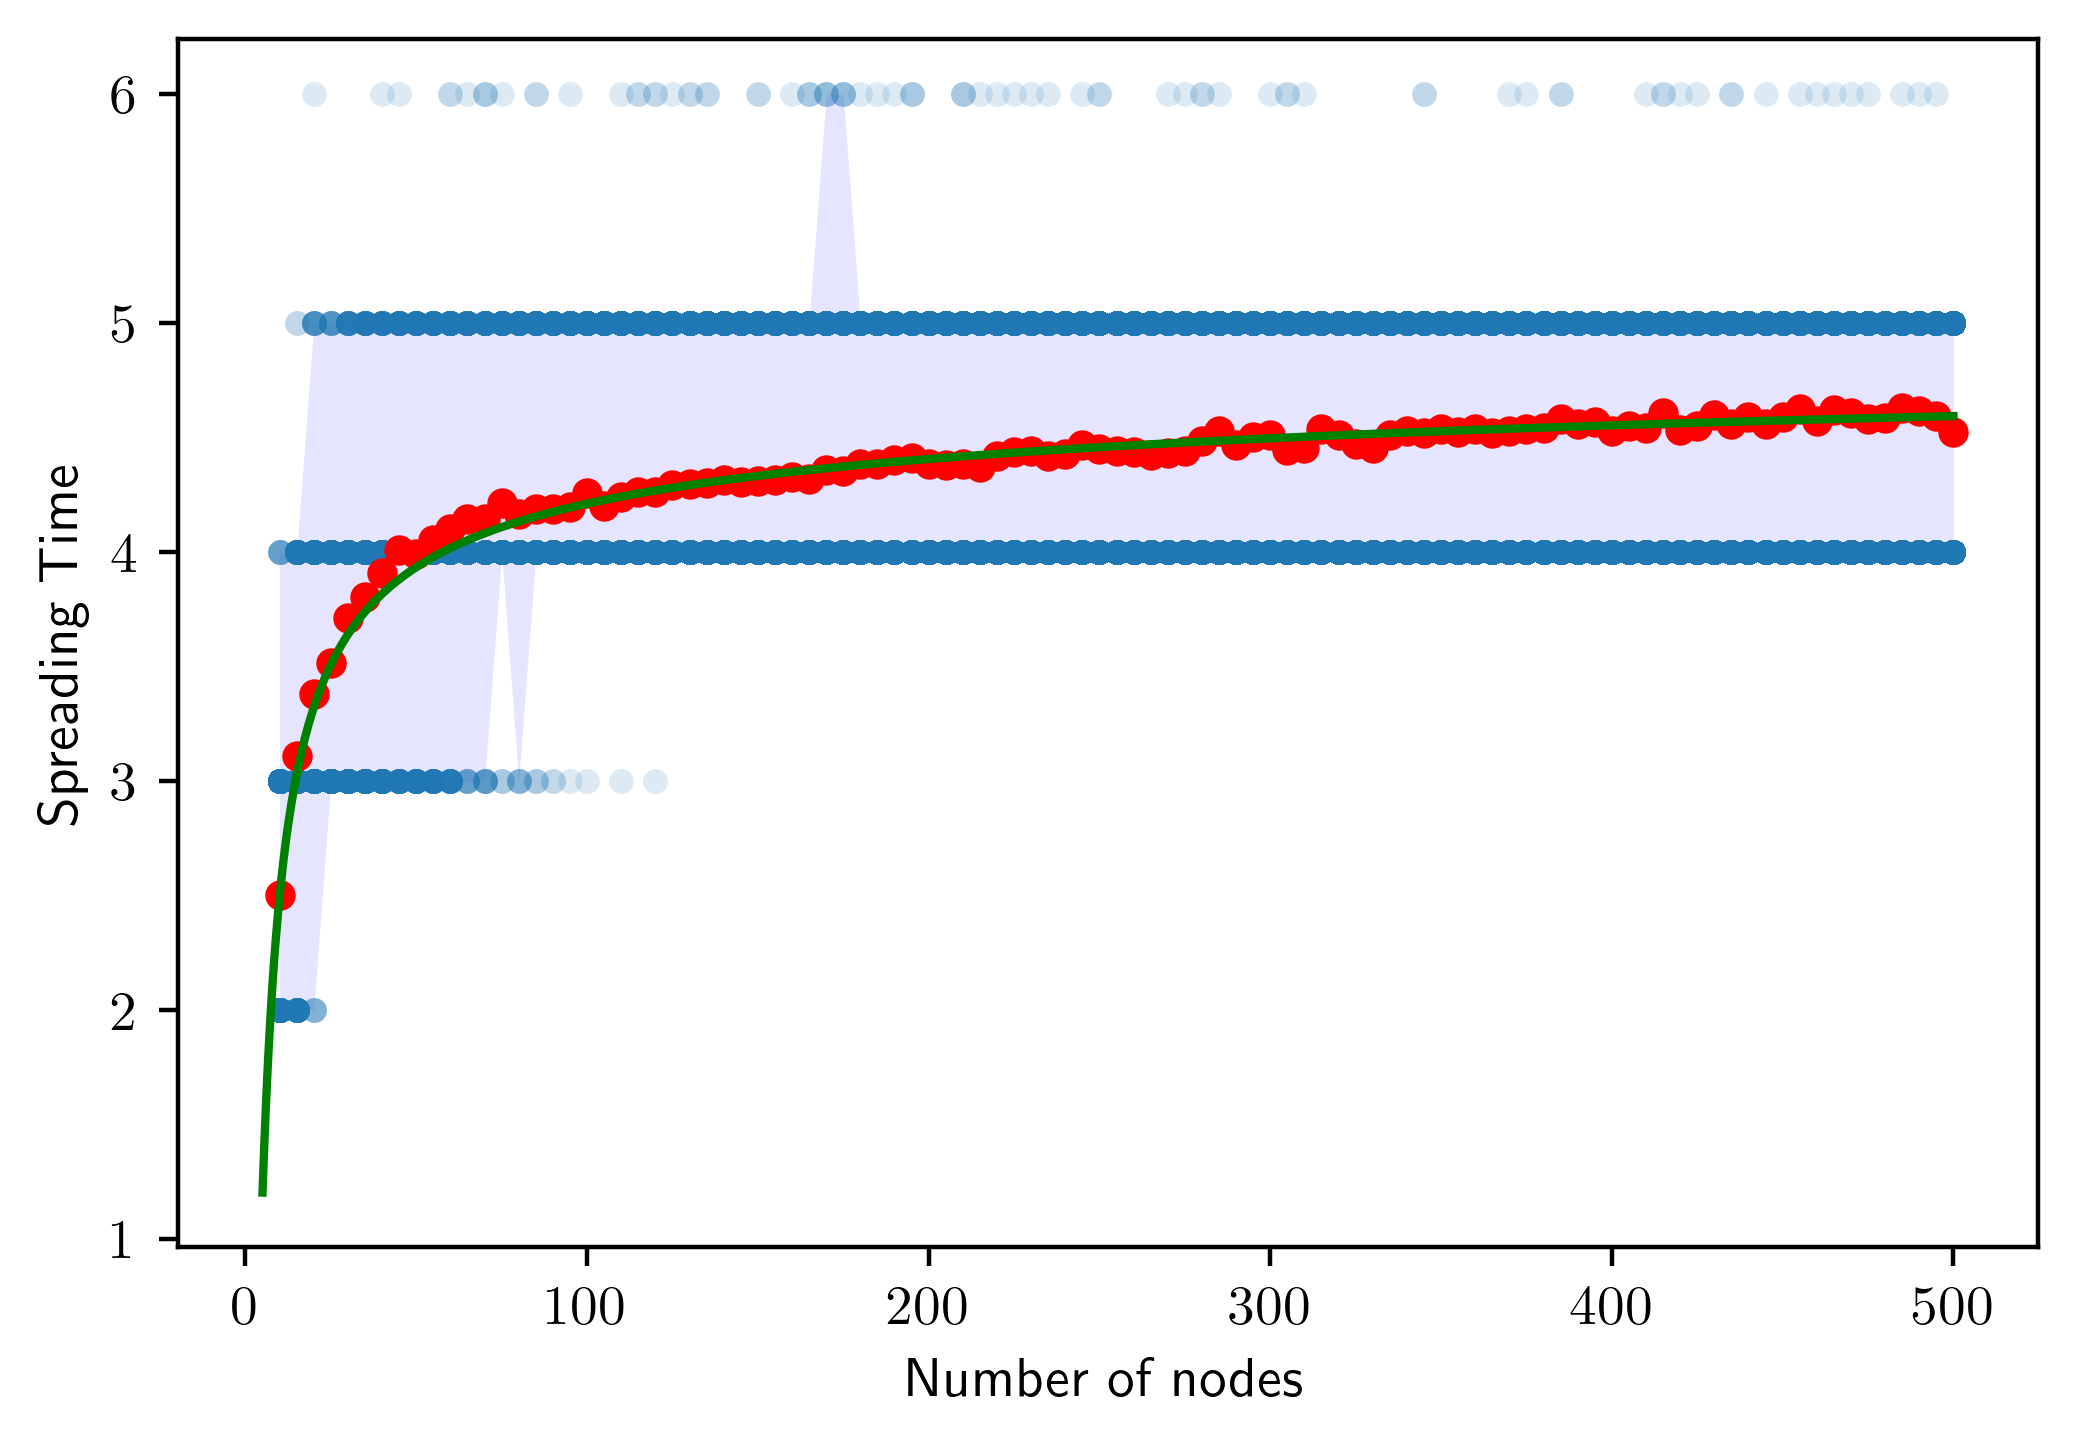
\includegraphics[width=1\textwidth]{./figures/flooding_simulation_first_term_max_p_over_4_with_errors.png}
	\caption{Results of Edge-Markovian Dynamic Network spreading time simulations when $\hat{p} = \frac{n^\frac{1}{\log \log n}}{4n}$}
	\label{fig:floodingSimFirstTermMaxPOver4}
\end{figure}

% TODO: TOP OF INTERVAL
Figure \ref{fig:floodingSimFirstTermMaxPOver4} displays the simulation results for rumour spread on the Stationary Edge-Markovian Network when $\hat{p} = \frac{n^\frac{1}{\log \log n}}{4n}$. This value of $\hat{p}$ was chosen since it has the same asymptotic scaling as the largest value of $\hat{p}$ for which Corollary \ref{corollary:edgeMarkovianThetaBound} holds. Since $\hat{p}$ is larger than in the simulations in Figure \ref{fig:floodingGnpSimResultsTight}, generally the network will have more edges, so we expect the spreading times to be shorter. This is exactly the behaviour we see for large $n$ in Figure \ref{fig:floodingSimFirstTermMaxPOver4}. Note also that the shape of the expected spreading time functions differs to Figure \ref{fig:floodingGnpSimResultsTight}, which reflects the change in $\hat{p}$. Note that again nearly all spreading times are within $\mathcal{O}(1)$of the mean, so we can reason about the growth of spreading times by comparing with the average spreading times. The expected spreading time again fits the simulated times well, due to Corollary \ref{corollary:edgeMarkovianThetaBound}.

\begin{figure}[h]
	\centering
	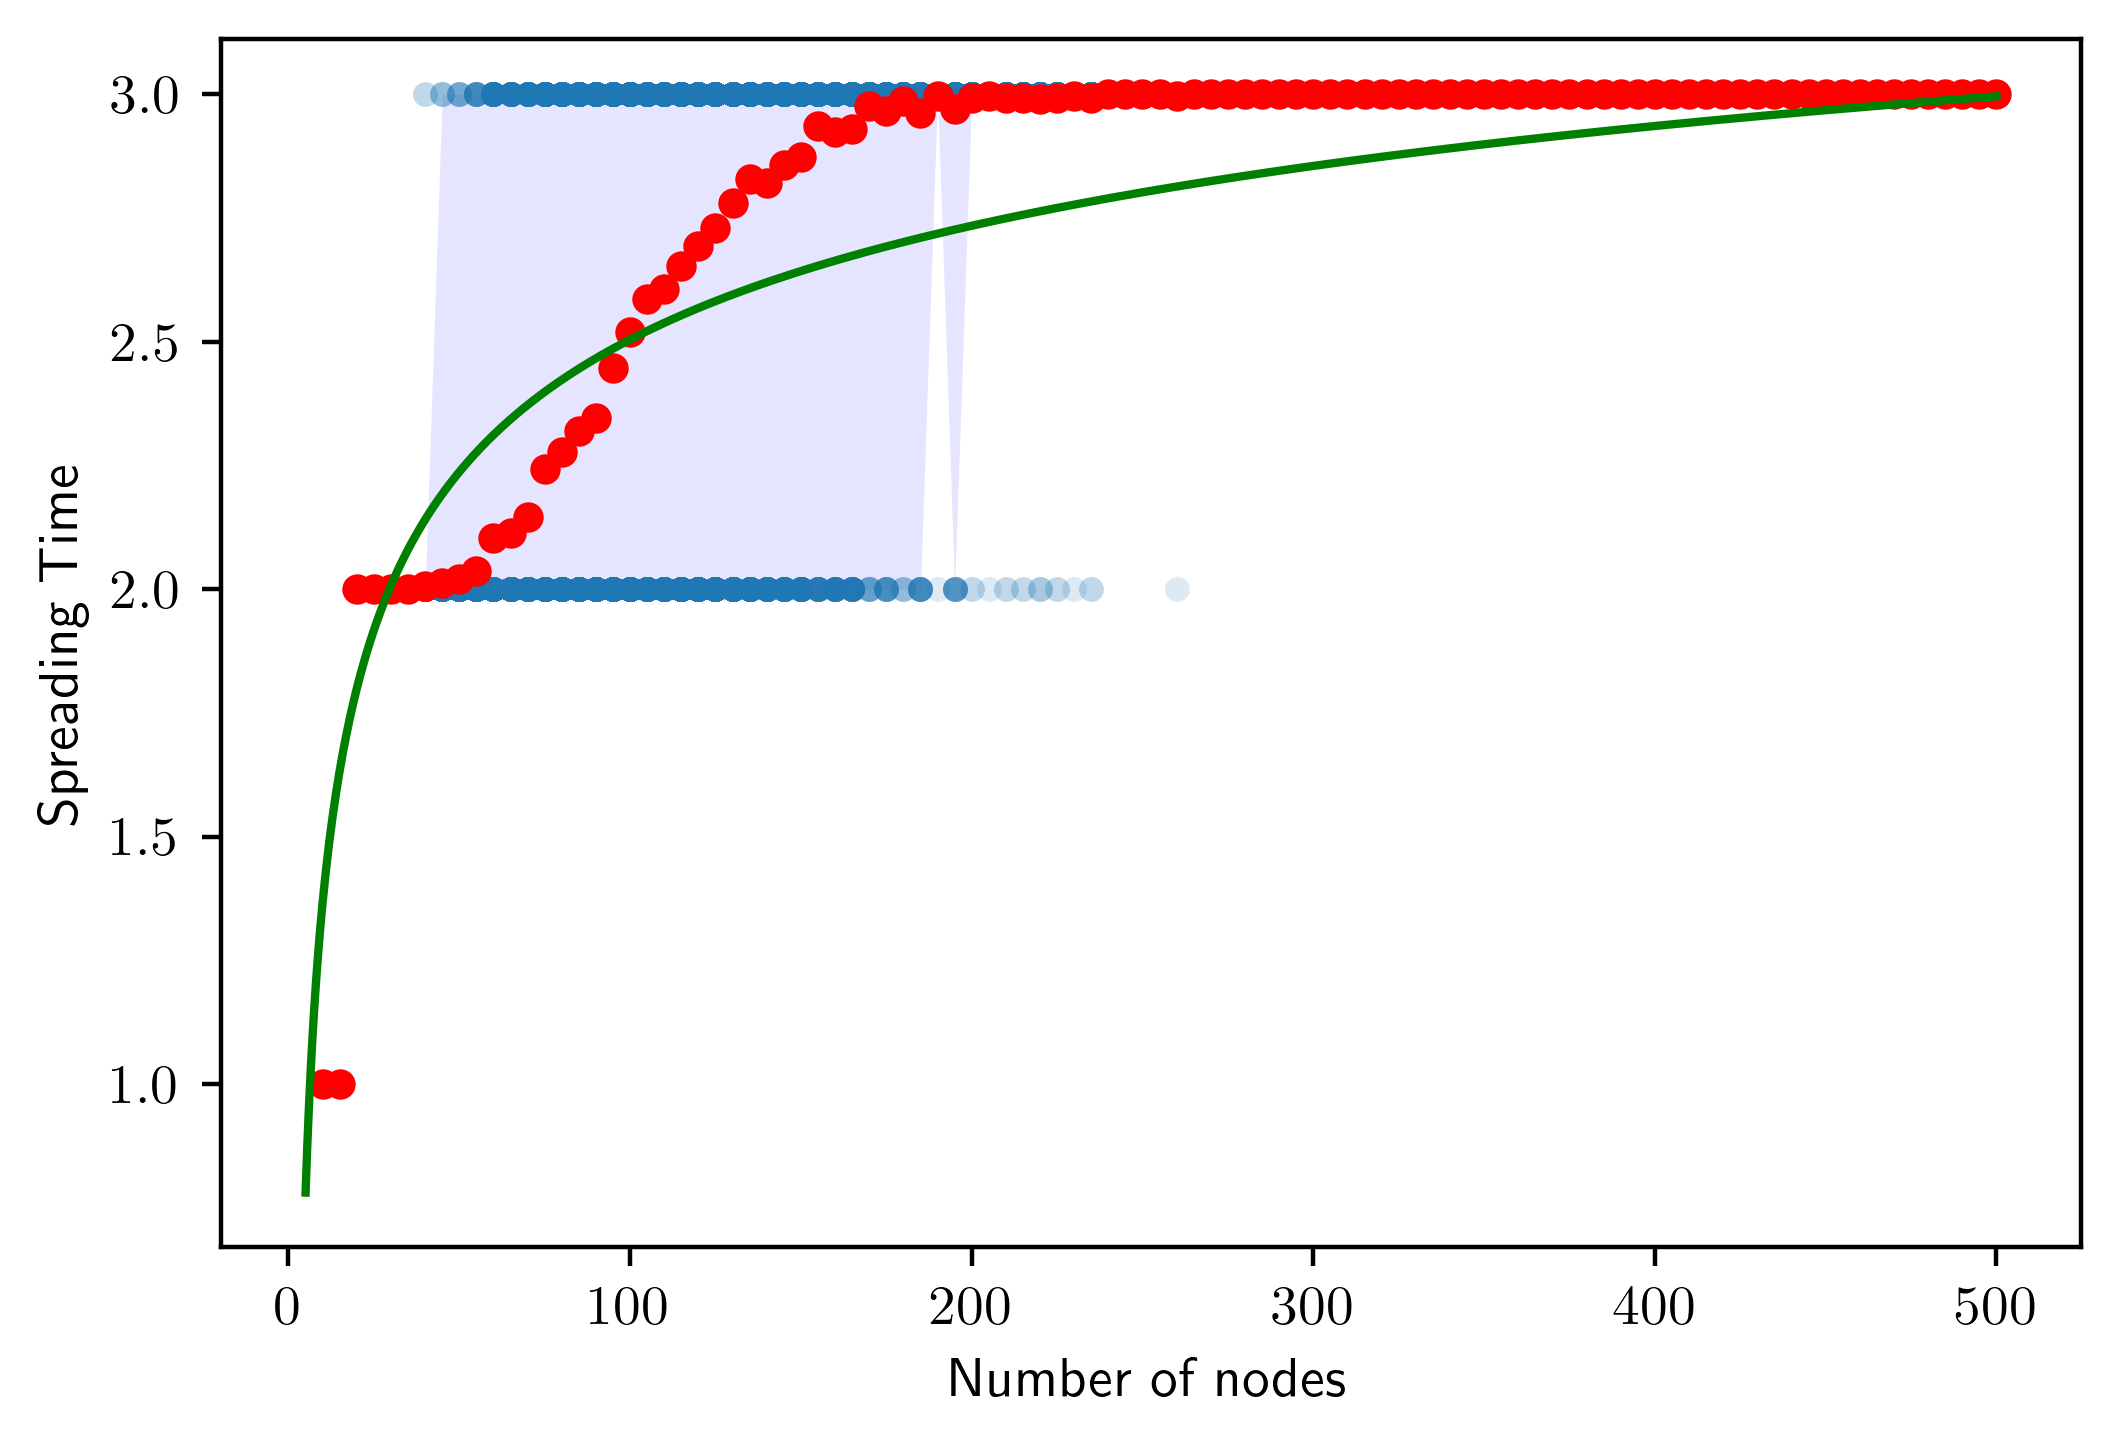
\includegraphics[width=1\textwidth]{./figures/flooding_simulation_first_term_max_p_with_errors.png}
	\caption{Results of Edge-Markovian Dynamic Network spreading time simulations when $\hat{p} = \frac{n^\frac{1}{\log \log n}}{n}$}
	\label{fig:floodingSimFirstTermMaxP}
\end{figure}

Figure \ref{fig:floodingSimFirstTermMaxP} shows the spreading time simulations when $\hat{p} = \frac{n^\frac{1}{\log \log n}}{n}$, the largest value of $\hat{p}$ for which Corollary \ref{corollary:edgeMarkovianThetaBound} holds. In this case, the expected growth function (displayed in green) is
$$
	g(n)
	= \Theta\left(\frac{\log n}{\log (n\hat{p})}\right) 
	= \Theta\left(\log \log n \right)
$$
We see that in this case the means do not fit the expected growth function as well as the previous two networks. We are not sure why this is the case, and could be an interesting area for further study. In Figure \ref{fig:floodingSimFirstTermMaxPOver4}, we saw that an equivalent function for $\hat{p}$ up to scaling constants closely fitted the mean spreading times. % TODO: What does this suggest?

A limitation of this analysis is that due to the size of $\hat{p}$, the spreading times are short, so it is difficult to identify the long-term growth of the spreading time even with values of $n$ up to 500. % TODO: IS THIS TRUE
% SUSPICIOUS OF THE GROWTH
This is exemplified in Figure \ref{fig:floodingSimFirstTermMaxP}, since the spreading time was 3 for all simulations with at least 250 nodes. In fact, even for networks with 10000 nodes, under this value of $\hat{p}$, we see found that the spreading time is consistently 3. We would like to explore this trend for larger networks to better characterise the growth rate of the spreading time. However, the computational cost of running such simulations was too great to produce statistically significant results, as we could not run enough such simulations in a reasonable time. Hence, another potential avenue for further study could be to implement more efficient simulations, to better charecterise the spreading time growth for large $n$. 


% TODO: Need larger values of n, computational cost for large networks, enough runs for statistical significance,
% saw that it holds for scaling proportional to this value of \hat{p}

% TODO: Tight in means, takes discrete values
% TODO: Refocus on answering a question - how well does it hold?

Overall, we established in Corollary \ref{corollary:edgeMarkovianThetaBound} that for values of $\hat{p}$ in the interval 
$$
	c \frac{\log n}{n} \leq \hat{p} \leq  \frac{n^\frac{1}{\log \log n}}{n}
$$
the bound given by Theorem \ref{theorem:edgeMarkovianFloodingBound} is tight. We verified this fact with simulations. However, for values of $\hat{p}$ at least as large as $\frac{n^\frac{1}{\log \log n}}{n}$, the spreading times from simulations are too small to characterise their growth. Hence, for $\hat{p}$ larger than $\frac{n^\frac{1}{\log \log n}}{n}$, we do not know how tightly the bound holds.